\documentclass[12pt,
border=1pt]{standalone}
\usepackage{pgfplots}
\usepackage{amsmath}
\usepackage{amssymb}

\pgfplotsset{compat=newest,
	width=6cm, height=5cm,
	xtick pos=left, ytick pos=left,
	%            scaled x ticks=real:1e-6,
}
% Kernel 2 FP64
\begin{document}
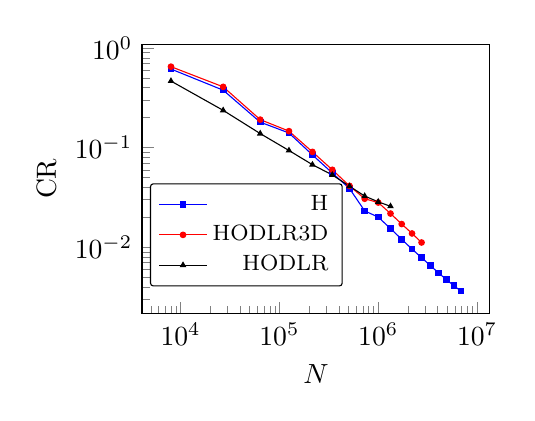
\begin{tikzpicture}[every mark/.append style={mark size=1pt}]
	\begin{axis}[	xlabel={$N$},
	ylabel={CR},
%		legend pos=south east,
		legend style={
                at={(0.3,0.1)},
               anchor=south,
               legend columns=1,
               cells={anchor=east},
               font=\footnotesize,
               rounded corners=1pt,
               },
		xmode = log,
	    ymode = log,
	   % xmin = 1e3,
	   % xmax = 1e6,
	   % ymin = 1e-10,
	   % ymax = 1e-0,
	   % xtick={1e-10, 1e-8, 1e-6,  1e-4,  1e-2},
	   % ytick={1e-8, 1e-6,  1e-4,  1e-2, 1e-0}
		]
		
		%Vaishnavi
		\addplot[
		color=blue,
		mark=square*,
		] coordinates {
(8000,0.617191)
(27000,0.378431)
(64000,0.180640)
(125000,0.140613)
(216000,0.084602)
(343000,0.055738)
(512000,0.038920)
(729000,0.023204)
(1000000,0.020078)
(1331000,0.015422)
(1728000,0.012008)
(2197000,0.009590)
(2744000,0.007856)
(3375000,0.006544)
(4096000,0.005493)
(4913000,0.004722)
(5832000,0.004102)
(6859000,0.003639)

		};
		%Zhao
		\addplot[
		color=red,
		mark=*,
		] coordinates {
(8000,6.518580e-01)
(27000,4.086700e-01)
(64000,1.914630e-01)
(125000,1.467360e-01)
(216000,9.079540e-02)
(343000,6.000270e-02)
(512000,4.135110e-02)
(729000,3.072480e-02)
(1000000,2.813110e-02)
(1331000,2.180600e-02)
(1728000,1.710970e-02)
(2197000,1.375910e-02)
(2744000,1.116820e-02)
		};
\addplot[
		color=black,
		mark=triangle*,
		] coordinates {
% (8000,0.472333)
% (27000,0.255545)
% (64000,0.182242)
% (125000,0.129209)
% (216000,0.108863)
% (343000,0.084138)
% (512000,0.071956)
% (729000,0.061018)
(8000,4.672540e-01)
(27000,2.372860e-01)
(64000,1.386410e-01)
(125000,9.374890e-02)
(216000,6.752820e-02)
(343000,5.325890e-02)
(512000,4.103130e-02)
(729000,3.269280e-02)
(1000000,2.859920e-02)
(1331000,2.578580e-02)
		};
		\legend{H, HODLR3D, HODLR}
		\end{axis}
\end{tikzpicture}
\end{document}